\documentclass{beamer}

\let\val\undefined
\usepackage{amsmath}
\usepackage{amsthm}
\usepackage{amsfonts}
\usepackage{grffile}
\usepackage{graphicx}
% for making a grid
%\usepackage[gridBG, gridunit=mm, gridcolor=blue!40, subgridcolor=blue!20]{eso-pic}


\usetheme[progressbar=frametitle]{metropolis}
\usepackage{libertine}

% *** Styles ***
%\setbeamertemplate{navigation symbols}{}
\usecolortheme{dolphin}
%\usecolortheme{rose}
%\setbeamercovered{transparent}
\usefonttheme{professionalfonts}
%\usefonttheme[onlymath]{serif}

% *** Colors ***
\newcommand{\tc}[2]{\textcolor{#1}{#2}}
\newcommand{\tcb}[1]{\tc{blue}{#1}}
\newcommand{\tcr}[1]{\tc{red}{#1}}
\newcommand{\tcg}[1]{\tc{green}{#1}}

\def\checkmark{\tikz\fill[scale=0.4](0,.35) -- (.25,0) -- (1,.7) -- (.25,.15) -- cycle;}

\newcommand{\Ex}{\mathbb{E}}
\newcommand{\E}{\mathbb{E}}
\newcommand{\Real}{\mathbb{R}}
\newcommand{\V}{\mathbb{V}}
\newcommand{\I}{\mathbb{I}}
\newcommand{\sd}{\operatorname{sd}}
\newcommand{\cov}{\operatorname{Cov}}
\newcommand{\corr}{\operatorname{corr}}
\renewcommand{\P}[1]{\mathbb{P}\left[#1\right]}
% \DeclareMathOperator{\Var}{Var}

\definecolor{varcolor}{RGB}{132,23,49}
\newcommand{\varname}[1]{\textcolor{varcolor}{\mathsf{#1}}}

\title{Probability 1}
\subtitle{MML 6.1}
\author{Samuel Carton (adapted from Marek Petrik)}
\date{8/2025}

\begin{document}
\begin{frame}
\maketitle
\end{frame}


\begin{frame} \frametitle{Probability Space}
\begin{itemize}
\item \textbf{Outcome space}: Set $\Omega$
  \vfill 
  % set of all possible outcomes
  % example: {J(ohn), E(ve), M(ary)}
\item \textbf{Event space} (sigma algebra): $\mathcal{F} \subset 2^{\Omega}$
  \vfill
  % all possible events, more than a single person can have a property
  % example {0, {J}, {E}, .., {J,E}, {J,M}, ..., {J,E,M}}
  % for finite \Omega, the set is typically a power set
\item \textbf{Probability function}: $P \colon \mathcal{F} \to [0,1]$
  % measures the probability of every student
  % could represent the probability of a student showing up for a class =
  % = relatively how often the student shows up for school
  % P(J) = 0.5, P(E) = 0.25, P(M) = 0.25
\end{itemize}
% \vfill \pause
% \textbf{Example}
% \begin{itemize}
% \item \textbf{Outcome space}: UNH students $\mathcal{U} = \{ \text{Jane}, \text{John}, \dots \}$ 
% \item \textbf{Even space}: All possible student groups: $2^{\mathcal{U}}$, must contain countable intersection, union, complement, and $\Omega$
% \item \textbf{Probability function}: $P(u), u \in \mathcal{U}$ probability of seeing a student $u$ on a random day on campus.
% \end{itemize}
% \vfill \pause
% \alert{What is the probability $P(\{u_1, u_2\})$ ($u_1 \neq u_2$)?}
% \pause
% \[ P(A \cup B) = P(A) + P(B) \text{ when } A \cap B = \emptyset  \]
\end{frame}

\begin{frame} \frametitle{Probability Space: Properties}
\begin{itemize}
\item \textbf{Outcome space}: Set $\Omega$
  \begin{itemize}
  \item Finite or infinite
  \end{itemize}
\item \textbf{Event space} (sigma algebra): $\mathcal{F} \subset 2^{\Omega}$
  \begin{itemize}
  \item Contains sample space:
  \item Closed under complements:
  \item Closed under countable unions:
  \item Closed under countable intersections:
  \end{itemize}
  \vfill 
\item \textbf{Probability measure}: $P \colon \mathcal{F} \to [0,1]$
  \begin{itemize}
  \item Mesure of sample space equals 1:
  \item Countably additive:
  \end{itemize}
  \vfill 
\end{itemize}
\end{frame}

\begin{frame} \frametitle{Random Variable}
  A $\mathcal{T}$-valued random variable $X$ (upper case!) is a function:
  \[ X \colon \Omega \to \mathcal{T}\]
    Examples \( \Omega = \{ J, E, M \} \):
    \vspace{4cm}
\end{frame}


\begin{frame} \frametitle{Random Variable: Common Types}
  \begin{enumerate}
  \item \textbf{Continuous (real-valued)}
   \vfill  
 \item \textbf{Discrete}
   \vfill 
  \end{enumerate}
\end{frame}

\begin{frame} \frametitle{Random Variable: Pre-image (inverse)}
  Pre-image \( X^{-1} \colon \mathcal{T} \to 2^{\Omega}  \) defined as
  \[
    X^{-1}(x) = \left\{ \omega \in \Omega \mid X(\omega) = x \right\} 
  \]
  Examples \( \Omega = \{ J, E, M \} \):
  \vspace{4cm} 
\end{frame}


\begin{frame} \frametitle{Probability Distribution}
  Always associated with a random variable for some $X\colon \Omega \to \mathcal{T}$
  \[
    \P{X = x} = P\left(X^{-1}(x)\right) = P \left(  \left\{ \omega \in \Omega \mid X(\omega) = x  \right\} \right)
  \]
  \vspace{4cm}
\end{frame}

\begin{frame}
  \frametitle{Probability Distributions}
  {\small Wikipedia is a good reference for their properties}\\
  \vfill
  \textbf{Discrete} random variable:
    \begin{itemize}
    \item Bernoulli: Heads or tails
    \item Binomial: Number of heads
    \item Geometric: Coin flips until heads
    \item Poisson: Number of customers 
    \end{itemize}
    \vfill 
    \textbf{Continuous} random variable:
    \begin{itemize}
    \item Normal: Central limit theorem
    \item Multivariate normal: Height and weight
    \item Laplace: Extreme weather events
    \end{itemize}
\end{frame}

\begin{frame} \frametitle{Regression vs Classification}
  Predicting target: $Y : \Omega \to \mathcal{T}$ \\
  \vfill
    \textbf{Regression}: continuous target \(\mathcal{T} = \Real \)
    \begin{itemize}
    \item Profits
    \item Probability of survival
    \end{itemize}
     \vfill  
    \textbf{Classification}: discrete target: \(\mathcal{T}\) is finite
    \begin{itemize}
    \item Color 
    \item State
    \item Year (could be either)
    \end{itemize}
\end{frame}

\begin{frame} \frametitle{Machine Learning Choices ...}
\centering
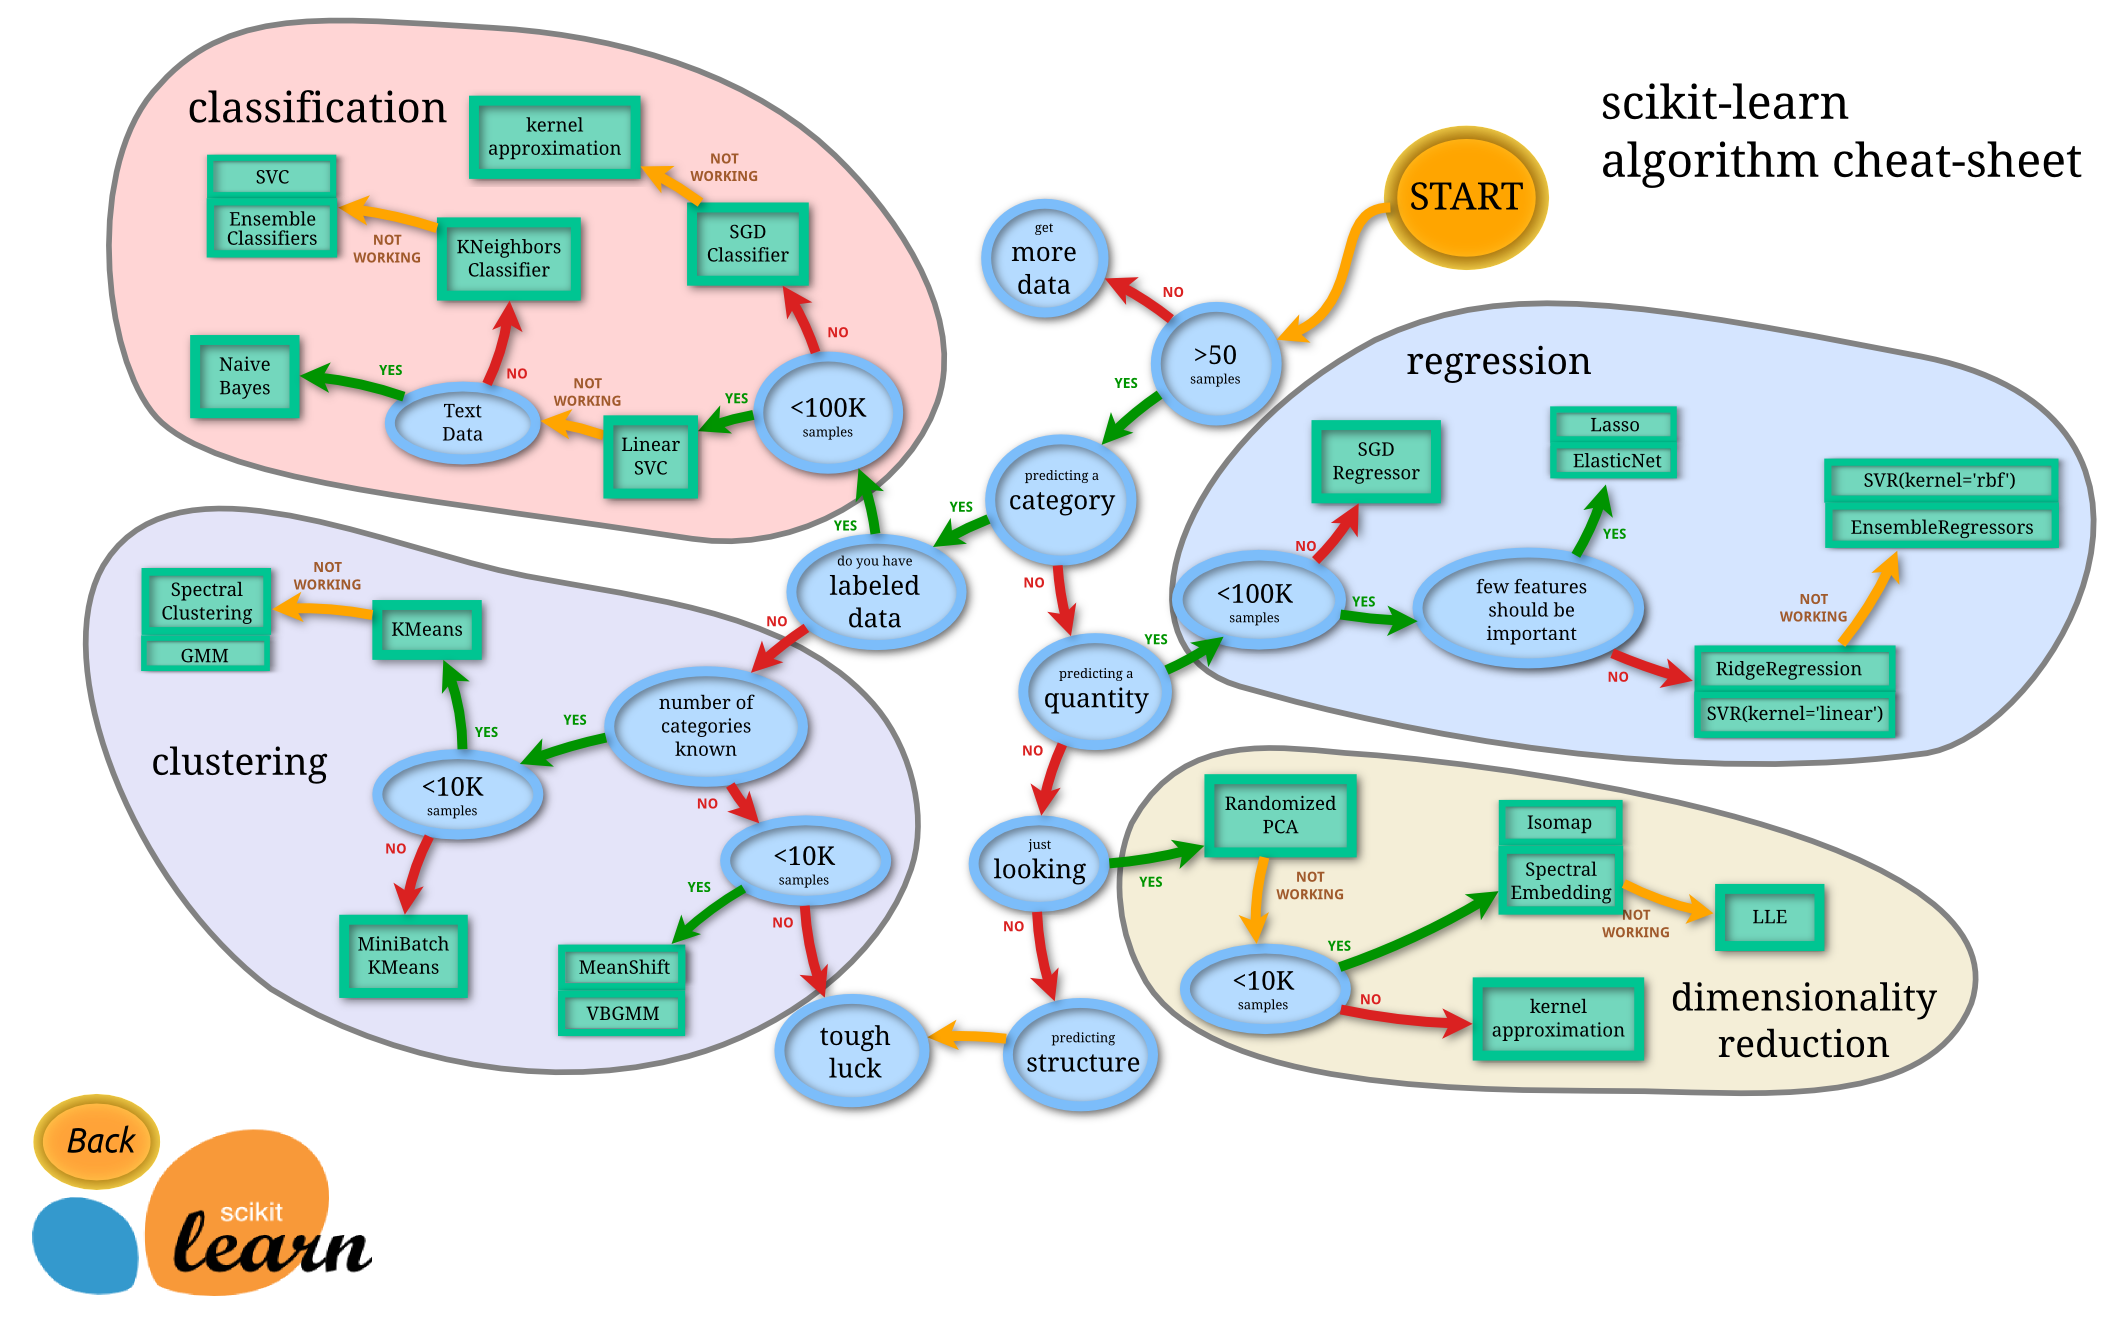
\includegraphics[width=\linewidth]{../figs/class1/ml_map.png}\\
{\tiny Source: \url{http://scikit-learn.org/stable/tutorial/machine_learning_map/index.html}} \\[3mm]
\end{frame}

% \begin{frame}
%   What is the probability that you see a student who is  7+ feet tall? \\
%   \vfill
%   Random variable is \emph{height}: $H$ \\
%   \vfill
%   \begin{align*}
%     \P[H \ge 7] &= P(H^{-1}(\{ h \in \Real \mid h \ge  7 \})) \\
%     &= P(\{ \omega \in \Omega  \mid H(\omega) \ge  7 \}) \\
%     &\approx \sum_{\omega \in \Omega } P(\omega) \cdot \I\{ H(\omega) \ge 7 \} 
%   \end{align*}
% \end{frame}


\end{document}

%%% Local Variables:
%%% mode: latex
%%% TeX-master: t
%%% End:
